%1372
\newpage
\subsection{絵を動かしてみよう}



今度は、表示した絵を動かしてみることにしましょう。

絵が動くことで、ゲームやアニメーションなどさらに\ruby{応用}{おう|よう}が広がります。

そのために覚えておかなければならないのが、\ruby{変数}{へん|すう}です。


変数について学んだことを覚えていますか?


\begin{description}
    \item \textgt{\bf \ \ (HSPのルール)}
    \item \textgt{\bf \ \ 「変数の名前=数値」で変数に値を入れることができる(代入)}
    \item \textgt{\bf \ \ 変数に数値を入れておくとパラメーターとして使える}
    \item \textgt{\bf \ \ mes命令の中で「+変数」を書くことで変数の中身を表示できる}
\end{description}

「a=100」と置くと、変数aに100という数字が記憶されます。

これを使って、いままで数字を書いていた部分に変数を代わりに書いて数字を変化させることができます。

スクリプトエディタの、ファイル→「開く」メニューから「fall.hsp」を読み込んで実行してみてください。



\begin{figure}[H]
    \begin{center}
      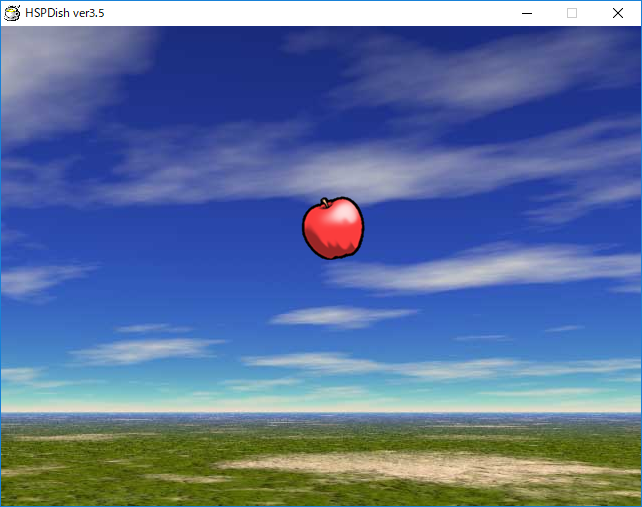
\includegraphics[keepaspectratio,width=9.183cm,height=7.241cm]{text04-img/s_fall.png}
      \caption{fall.hspの実行画面}
    \end{center}
    \label{fig:prog_menu}
\end{figure}

今度はリンゴが動いているのがわかると思います。


\begin{figure}[H]
    \begin{center}
      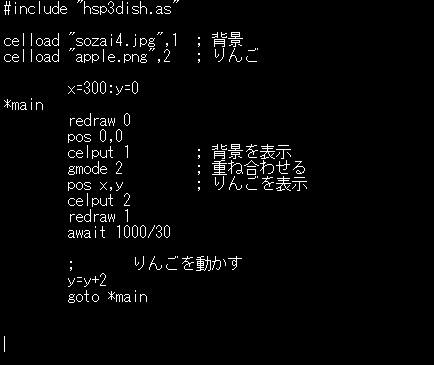
\includegraphics[keepaspectratio,width=10.954cm,height=9.213cm]{text04-img/text04-img020.png}
    \end{center}
    \label{fig:prog_menu}
\end{figure}


プログラムを見てみましょう。

変数xと変数yが、リンゴの横、縦の位置を\ruby{記憶}{き|おく}しています。

最初に「x=300:y=0」の行で、変数xに300を、変数yに0を\ruby{代入}{だい|にゅう}しています。



\begin{description}
    \item \textgt{\bf \ \ (HSPのルール)}
    \item \textgt{\bf 「:」の\ruby{記号}{き|ごう}を入れると、行を分けたのと同じように別な命令を書ける}
    \item \textgt{\bf \ \ 「:」の記号を使って1行にたくさんの命令を書くことができる}
\end{description}

「pos x,y」がありますので、celputする時の位置を変数x,yで変えられるようになっています。

つまり、横の位置が変数x、縦の位置が変数yに記憶されていることになります。

実際にリンゴの位置を変えているのが、「y=y+2」の部分です。

ここを繰り返し実行することで、変数yの値が2ずつ増えていきます。


\begin{description}
    \item \textgt{\bf \ \ (HSPのルール)}
    \item \textgt{\bf \ \ 「数式とは、数値と変数、またはそれらを計算式でつなげて書くこと}
    \item \textgt{\bf \ \ 「+」は足し算、「-」は引き算、「*」は掛け算(×)、「/」は割り算(÷) }
\end{description}



「y=y+2」は変数yに記憶されている数字に2を足すという意味だと覚えておきましょう。

これで、縦の位置が少しずつ変化するようになります。
\newpage
\subsection{例題に挑戦しよう}


終わってしまった人は、以下の例題にも挑戦してみよう。

・色々な動きに挑戦してみよう

・自分で用意した絵を動かして表示する

例題の考え方がわからない時は、近くのTAか先生に聞いてください。

わからない所は、そのままにせず、必ず答えを見つけてから先に進みましょう。

%1522


